\documentclass{standalone}
\usepackage{tikz}
\usepackage{ctex,siunitx}
\setCJKmainfont{Noto Serif CJK SC}
\usepackage{tkz-euclide}
\usepackage{amsmath,mhchem}
\usetikzlibrary{patterns, calc}
\usetikzlibrary {decorations.pathmorphing, decorations.pathreplacing, decorations.shapes,}
\begin{document}
\small
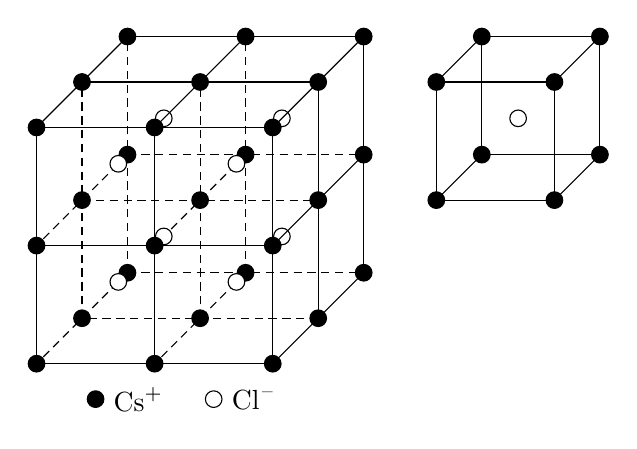
\begin{tikzpicture}[>=stealth,scale=1.5]
  % \useasboundingbox(-1,-2)rectangle(8,6);
  \draw[densely dashed] (0,0,0)--(0,0,2);
  \draw[densely dashed] (0,0,0)--(0,2,0);
  \draw[densely dashed] (0,0,0)--(2,0,0);
  \draw[densely dashed] (0,1,0)--(0,1,2);
  \draw[densely dashed] (0,1,0)--(2,1,0);
  \draw[densely dashed] (1,1,0)--(1,1,2);
  \draw[densely dashed] (1,0,0)--(1,2,0);
  \draw[densely dashed] (1,0,0)--(1,0,2);
  \draw[densely dashed] (0,1,1)--(2,1,1);
  \draw[densely dashed] (2,0,1)--(0,0,1);
  \draw[densely dashed] (1,0,1)--(1,2,1);
  \draw[densely dashed] (0,0,1)--(0,2,1);
  \foreach \x in {0,1,2}
  \foreach \y in {0,1,2}
  {
  \draw [fill=black](\x,\y,0) circle (2pt);
  }
  \foreach \x in {0.5,1.5}
  \foreach \y in {0.5,1.5}
  {
  \draw [fill=white](\x,\y,0.5) circle (2pt);
  }
  \foreach \x in {0,1,2}
  \foreach \y in {0,1,2}
  {
  \draw [fill=black](\x,\y,1) circle (2pt);
  }
  \foreach \x in {0.5,1.5}
  \foreach \y in {0.5,1.5}
  {
  \draw [fill=white](\x,\y,1.5) circle (2pt);
  }
  \foreach \x in {0,1,2}
  \foreach \y in {0,1,2}
  {
  \draw [fill=black](\x,\y,2) circle (2pt);
  }
  \draw[] (0,2,0)--(0,2,2);
  \draw[] (0,2,0)--(2,2,0);
  \draw[] (1,2,0)--(1,2,2);
  \draw[] (2,1,0)--(2,1,2);
  \draw[] (2,2,0)--(2,2,2);
  \draw[] (2,0,0)--(2,0,2);
  \draw[] (2,0,0)--(2,2,0);
  \draw[] (0,2,1)--(2,2,1);
  \draw[] (0,2,2)--(2,2,2);
  \draw[] (0,1,2)--(2,1,2);
  \draw[] (0,2,2)--(0,0,2);
  \draw[] (2,0,2)--(0,0,2);
  \draw[] (2,0,2)--(2,2,2);
  \draw[] (2,0,1)--(2,2,1);
  \draw[] (1,0,2)--(1,2,2);
  % \foreach \x in {0,1,2}
  % \foreach \y in {0,1,2}
  % \foreach \z in {0,1,2}
  % {
  % \draw [fill=black](\x,\y,\z) circle (2pt);
  % }
  % \foreach \x in {0.5,1.5}
  % \foreach \y in {0.5,1.5}
  % \foreach \z in {0.5,1.5}
  % {
  % \draw [fill=white](\x,\y,\z) circle (2pt);
  % }
  \draw [fill=white] ( 1.5,-0.3,2 )  circle (2pt)node[right=3pt]{\ce{Cl-}};
  \draw [fill=black] ( 0.5,-0.3,2 )  circle (2pt)node[right=3pt]{\ce{Cs+}};
  \foreach \x in {3,4}
  \foreach \y in {1,2}
  \foreach \z in {0,1}
  {
  \draw [fill=black](\x,\y,\z) circle (2pt);
  }
  \draw(3,1,0)--(4,1,0);
  \draw(3,2,0)--(4,2,0);
  \draw(3,1,1)--(4,1,1);
  \draw(3,2,1)--(4,2,1);
  \draw(4,1,0)--(4,2,0);
  \draw(4,1,0)--(4,2,0);
  \draw(3,1,0)--(3,2,0);
  \draw(3,1,1)--(3,2,1);
  \draw(4,1,1)--(4,2,1);
  \draw(4,2,0)--(4,2,1);
  \draw(3,2,0)--(3,2,1);
  \draw(4,1,0)--(4,1,1);
  \draw(3,1,0)--(3,1,1);
  \draw(3.5,1.5,0.5)circle(2pt);
\end{tikzpicture}
\end{document}